Over a linear search, almost all search methods perform worse in indexing.
We therefore provide a few quick summarative statistics concerning indexing.
It took 15 minutes and 41 seconds to do a cold index of the considered Go standard library.
The \texttt{log} package, fairly representative in terms of amount fragments contained,
took 423 milliseconds to index. 
It is likely that the steady state of such a search engine in the wild would index the standard library and each individual package.
This is because users will often want to query things such has how to convert some data type into another, often a package specific query.
So, while certainly longer than indexing by trigrams, it seems that times for indexing are not too high.

We will give an overview of the performance of the querying of types in the below.
A key evaluation is whether using a VP-Tree for code search is a true performance gain over a linear method.
To test this we compared the time for a linear query (cutoff at max value $1000$) under various other cutoffs ($1$ and $100$).
We plotted the speed of querying with a $1$ for a cutoff over linear speed in Figure \ref{dist1plot},
and similarly with a speed of $6$ in Figure \ref{dist6plot}.
In these plots we can see that when querying with a cutoffs of $1$, 120 of the 130 benchmarks saw a speed up,
and just a little worse for cutoffs of $6$.
Additionally, for a little over two thirds of the benchmarks we at least haved the time of a linear search.
And, those benchmarks that went over did so by often very little.
What accounts for the over run?
Often it is packages like \texttt{internal/cfg}, \texttt{go/format} and \texttt{crypto/internal} packages that have very few functions,
and so prone to high variance fron noise.

In figure \ref{allplot} we show the performance of all the packages run together.
We can see serious speed up gains for cutoffs of size less than or equal to $5$,
after which speed up is negligable at further distances.
This likely because large swathes of objects often become within range at further distances such as functions and various constants.
This means that the index of the tree becomes less useful as we as all subsections are explored as they are mostly within 
a ball of cutoff $10$ for some query target. 

We conclude that indexing can often get often order of magnitude improvements over linear searchs,
so \textbf{RQ1} can be answered: 
yes they are effective at reducing time complexity of problems.

\begin{figure}
    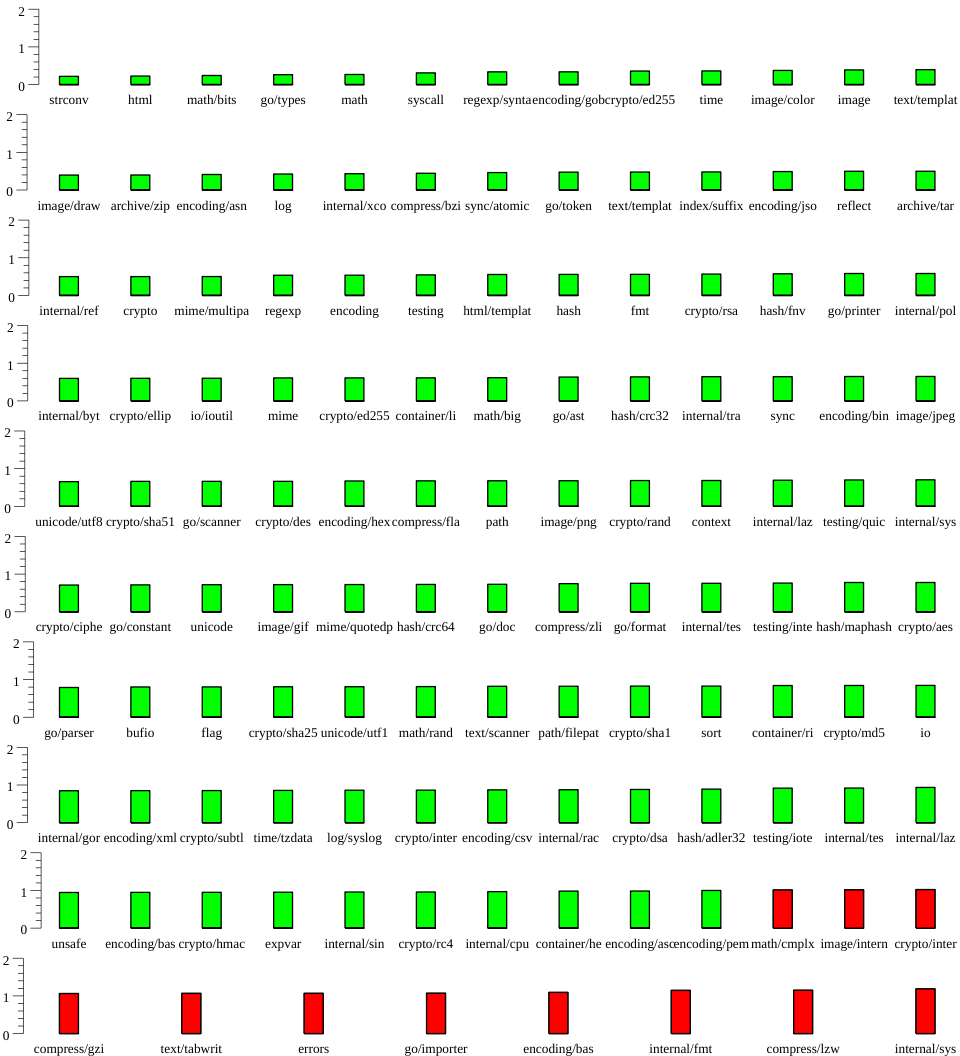
\includegraphics[width=\textwidth]{example1.png}
    \label{dist1plot}
    \centering
    \caption{Each Go module was indexed and then randomly queried.
    Speed up over linear search for a search distance of $1$ is plotted for each Go module.
    Green idicates search was fater, red otherwise.
    Names are the first twelve characters of module name.
    The rest are elided for readability.}
\end{figure}
\begin{figure}
    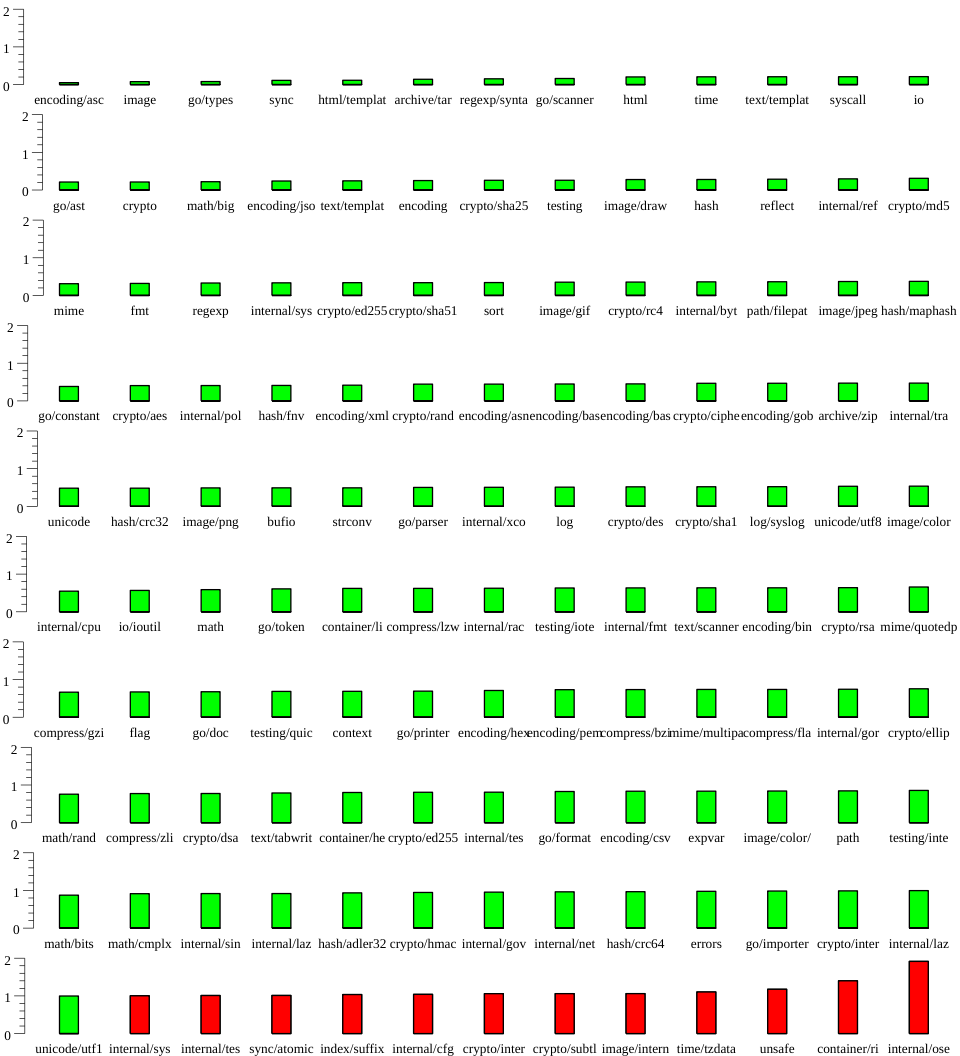
\includegraphics[width=\textwidth]{example6.png}
    \label{dist6plot}
    \centering
    \caption{Each Go module was indexed and then randomly queried.
    Speed up over linear search for a search distance of $6$ is plotted for each Go module.
    Green idicates search was fater, red otherwise.
    Names are the first twelve characters of module name.
    The rest are elided for readability.}
\end{figure}
\begin{figure}
    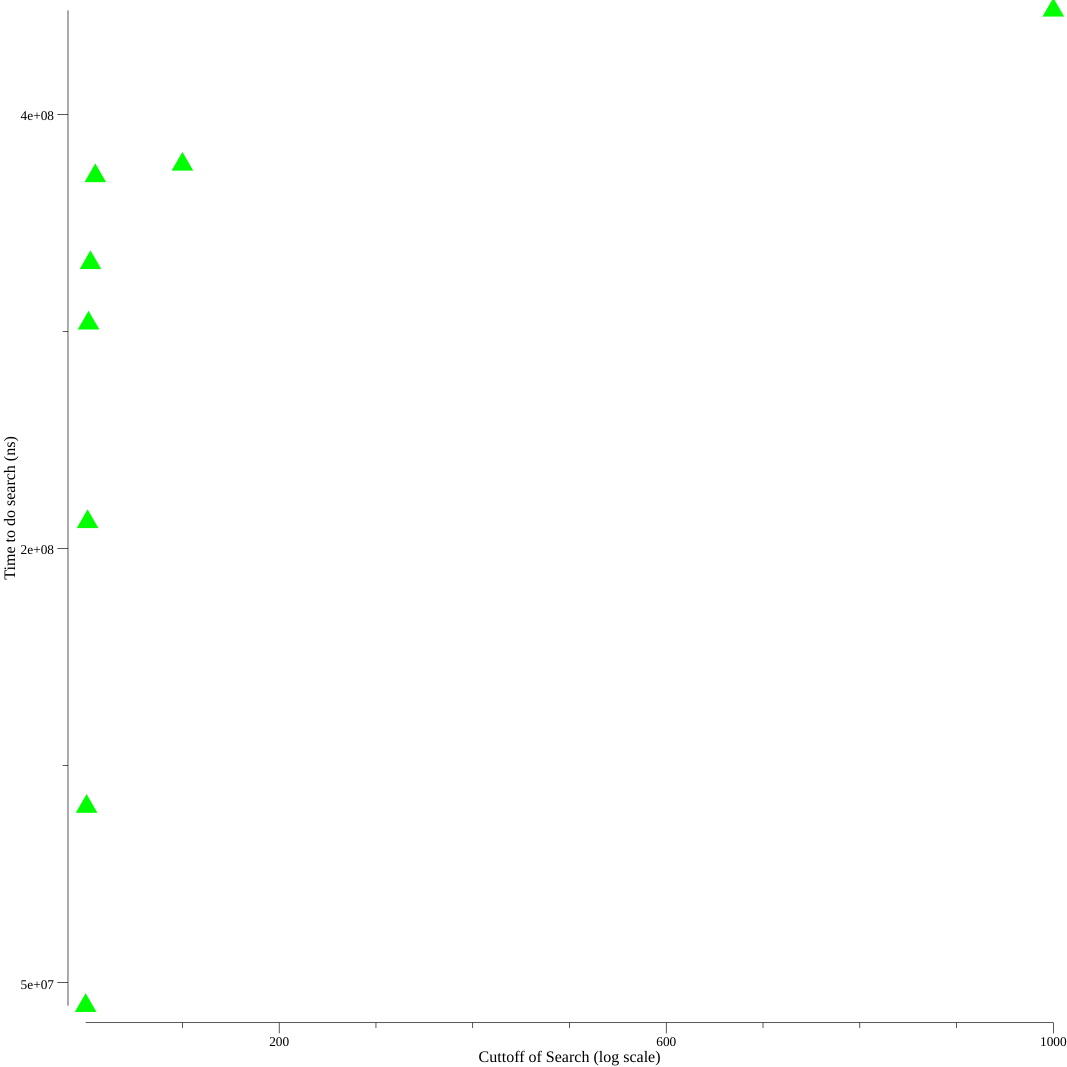
\includegraphics[width=0.5\textwidth]{alldat.png}
    \label{allplot}
    \centering 
    \caption{Query times indexing on all data}
\end{figure}